\documentclass{article}

% Some useful packages.
\usepackage{amsmath}
\usepackage{siunitx}
\usepackage{graphicx}
\usepackage{verbatim}
\usepackage{mhchem}

% Reduces margins substantially.
\usepackage{geometry}
\newgeometry{margin=2.5cm}

% Allows headers and footers.
\usepackage{fancyhdr}
\pagestyle{fancy}
% Get rid of annoying line under header.
\renewcommand{\headrulewidth}{0pt}

\lhead{}
\chead{BTTM8 - CLIMATE MODELLING - USING HADAM3 TO MODEL CLIMATE CHANGE}
\rhead{}
%\lfoot{}
%\cfoot{}
%\rfoot{}

\usepackage[backend=bibtex,style=authoryear,sorting=nyt,dashed=false]{biblatex}
\bibliography{references/references}
\renewcommand*{\nameyeardelim}{\addcomma\space}

% 2500 words max.
% Table of information about your simulation (as appendix): 10%
% Discussion of climate model: 15%
% Presentation of experimental results: 30%
% Discussion of experiment: 30%
% Use of wider literature: 5%
% General structure: 10%

% Analysing_your_runs
% Converting_UM_files
% Course_work_guide
% geogg134merit
% geogg134pass
% Setting_up_your_runs
% marengoInternal
% WG1AR5_ALL_FINAL
% WG1AR5_AnnexI_FINAL
% WG1AR5_Chapter02_FINAL
% WG1AR5_Chapter06_FINAL
% WG1AR5_Chapter08_FINAL
% WG1AR5_Chapter09_FINAL
% WG1AR5_Chapter14_FINAL
% WG1AR5_SPM_FINAL
% WG1AR5_TS_FINAL
% SREX-All_FINAL
% RCP_Guide
% SREX-Ch3-Supplement_FINAL

\begin{document}

\part*{Using HadAM3 to model the effects of climate change}

\section*{Abstract}

\ce{CO2} climate sensitivity (\SI{}{W.m^{-2}.K^{-1}})

\section{Introduction}

According to \textcite{gregory2004new}, you can never have to much sensitivity. Last year's ref: \parencite{geogg134merit}.

IPCC ref: \parencite{WG1AR5_Chapter02_FINAL}

\section{Methods}

\subsection{Model}

\section{Results}

\begin{figure}[hbp]
    \centering
    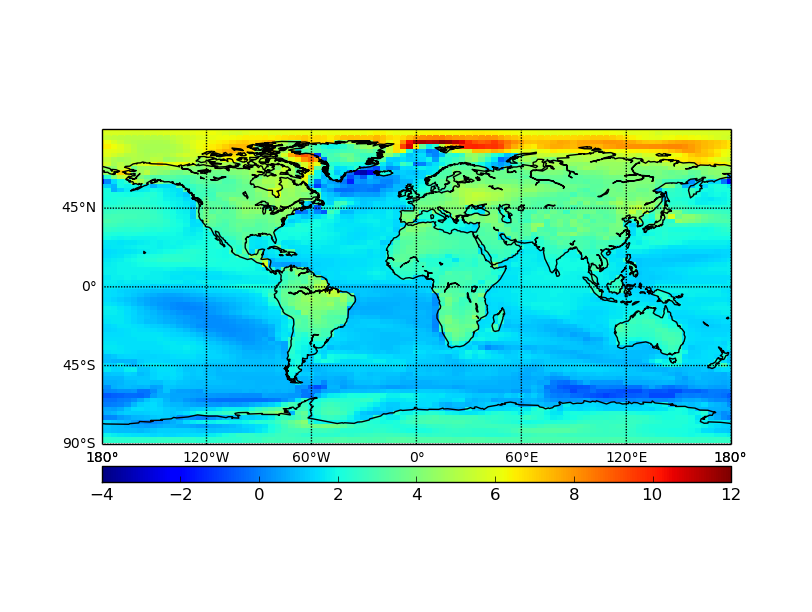
\includegraphics[width=\textwidth]{figures/figure_1}
    \caption{Caption.}
    \label{fig:figure_1}
\end{figure}

\section{Discussion}

\section{Conclusions}

\printbibliography
\appendix 

\section{Required output}

\begin{enumerate}
    \item first
    \item first
    \item first
    \item second
    \item second
\end{enumerate}

\end{document}
